\section{Analysis Models}
These models serve as conceptual designs and are later used when it comes to
concrete implementations.

\subsection{Behavioral modules and interaction}
\begin{figure}[htb]
\centering
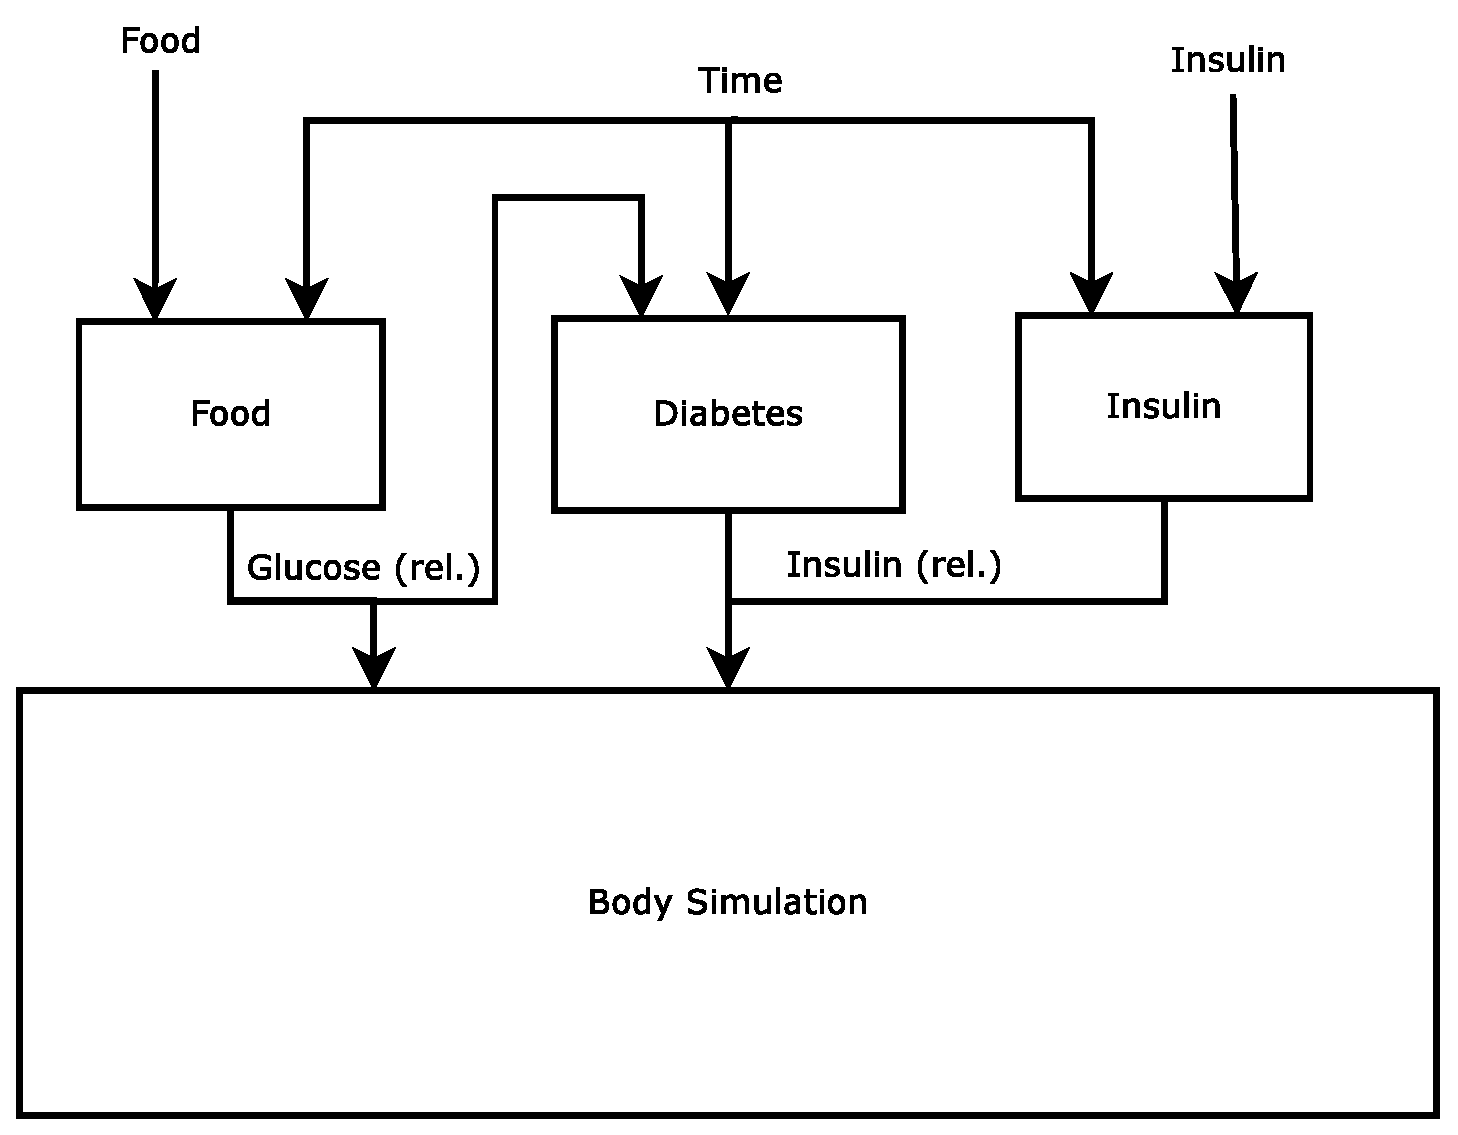
\includegraphics[scale=0.4]{images/Analysis_Model}
\caption{Analysis model of behavioral modules and theire interaction}
\label{fig:analysis_model_behavioral_modules}
\end{figure}

\newpage
\subsection{Body simulation (aka: putting behavioral modules together)}
The body simulation must combine the three behavioral modules and provide
inputs and outputs to these.
Such in- and outputs include but are not limited to GUIs and reading/writing
from/to CSV-Files.
A first conceptual design can look as follows (see
\vref{fig:body_sim_analysis_model}):

\begin{figure}[htb]
\centering
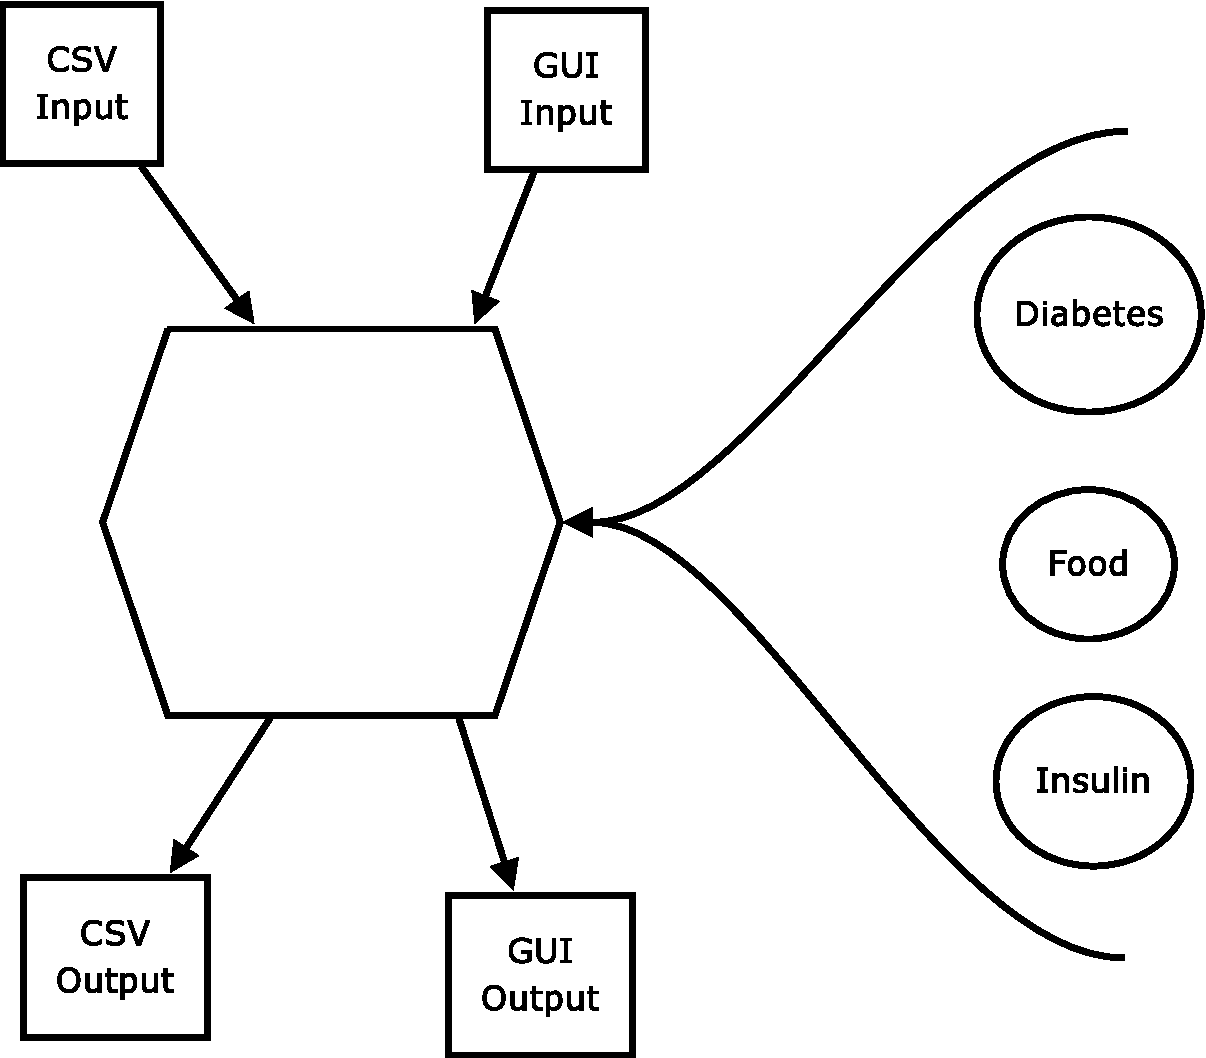
\includegraphics[scale=0.4]{images/Body_Simulation_analysis_model.pdf}
\caption{Body simulation analysis model}
\label{fig:body_sim_analysis_model}
\end{figure}